
\documentclass[simplex.tex]{subfiles}
% NO NEED TO INPUT PREAMBLES HERE
% packages are inherited; you can compile this on its own

\begin{document}
\subsection{fngs}

Through the fngs pipeline, we develope a robust processing pipeline and web service for providing automated acquisition of functional connectomes from structural and functional MRI. The fngs pipeline was developed around the glass-box principle; each step of the pipeline produces intuitive and descriptive quality assurance so users can be confident that the internals of the pipeline are performing properly. We provide an open-source docker container, links to all code, and have numerous tutorials and demos available \href{https://github.com/neurodatadesign/fngs}{Tutorials} for users to receive a step-by-step introduction to the pipeline. Moreover, we provide an interactive schematic of the pipeline \href{https://neurodatadesign.github.io/fngs/about_fngs/Schematic.html}{Schematic}. Note that the headings in each box at the bottom link to the documentation for the respective steps of the pipeline. Using the one-click cloud deployment of fngs, we were able to analyze 1200 human connectomes in 7 hours for a total of \$80. The cloud deployment procedure of the fngs pipeline can be seen in Figure (\ref{fig:fngs-workflow}).

\begin{figure}[h!]
\begin{cframed}[lgray]
\centering
\begin{subfigure}[h]{1\textwidth}
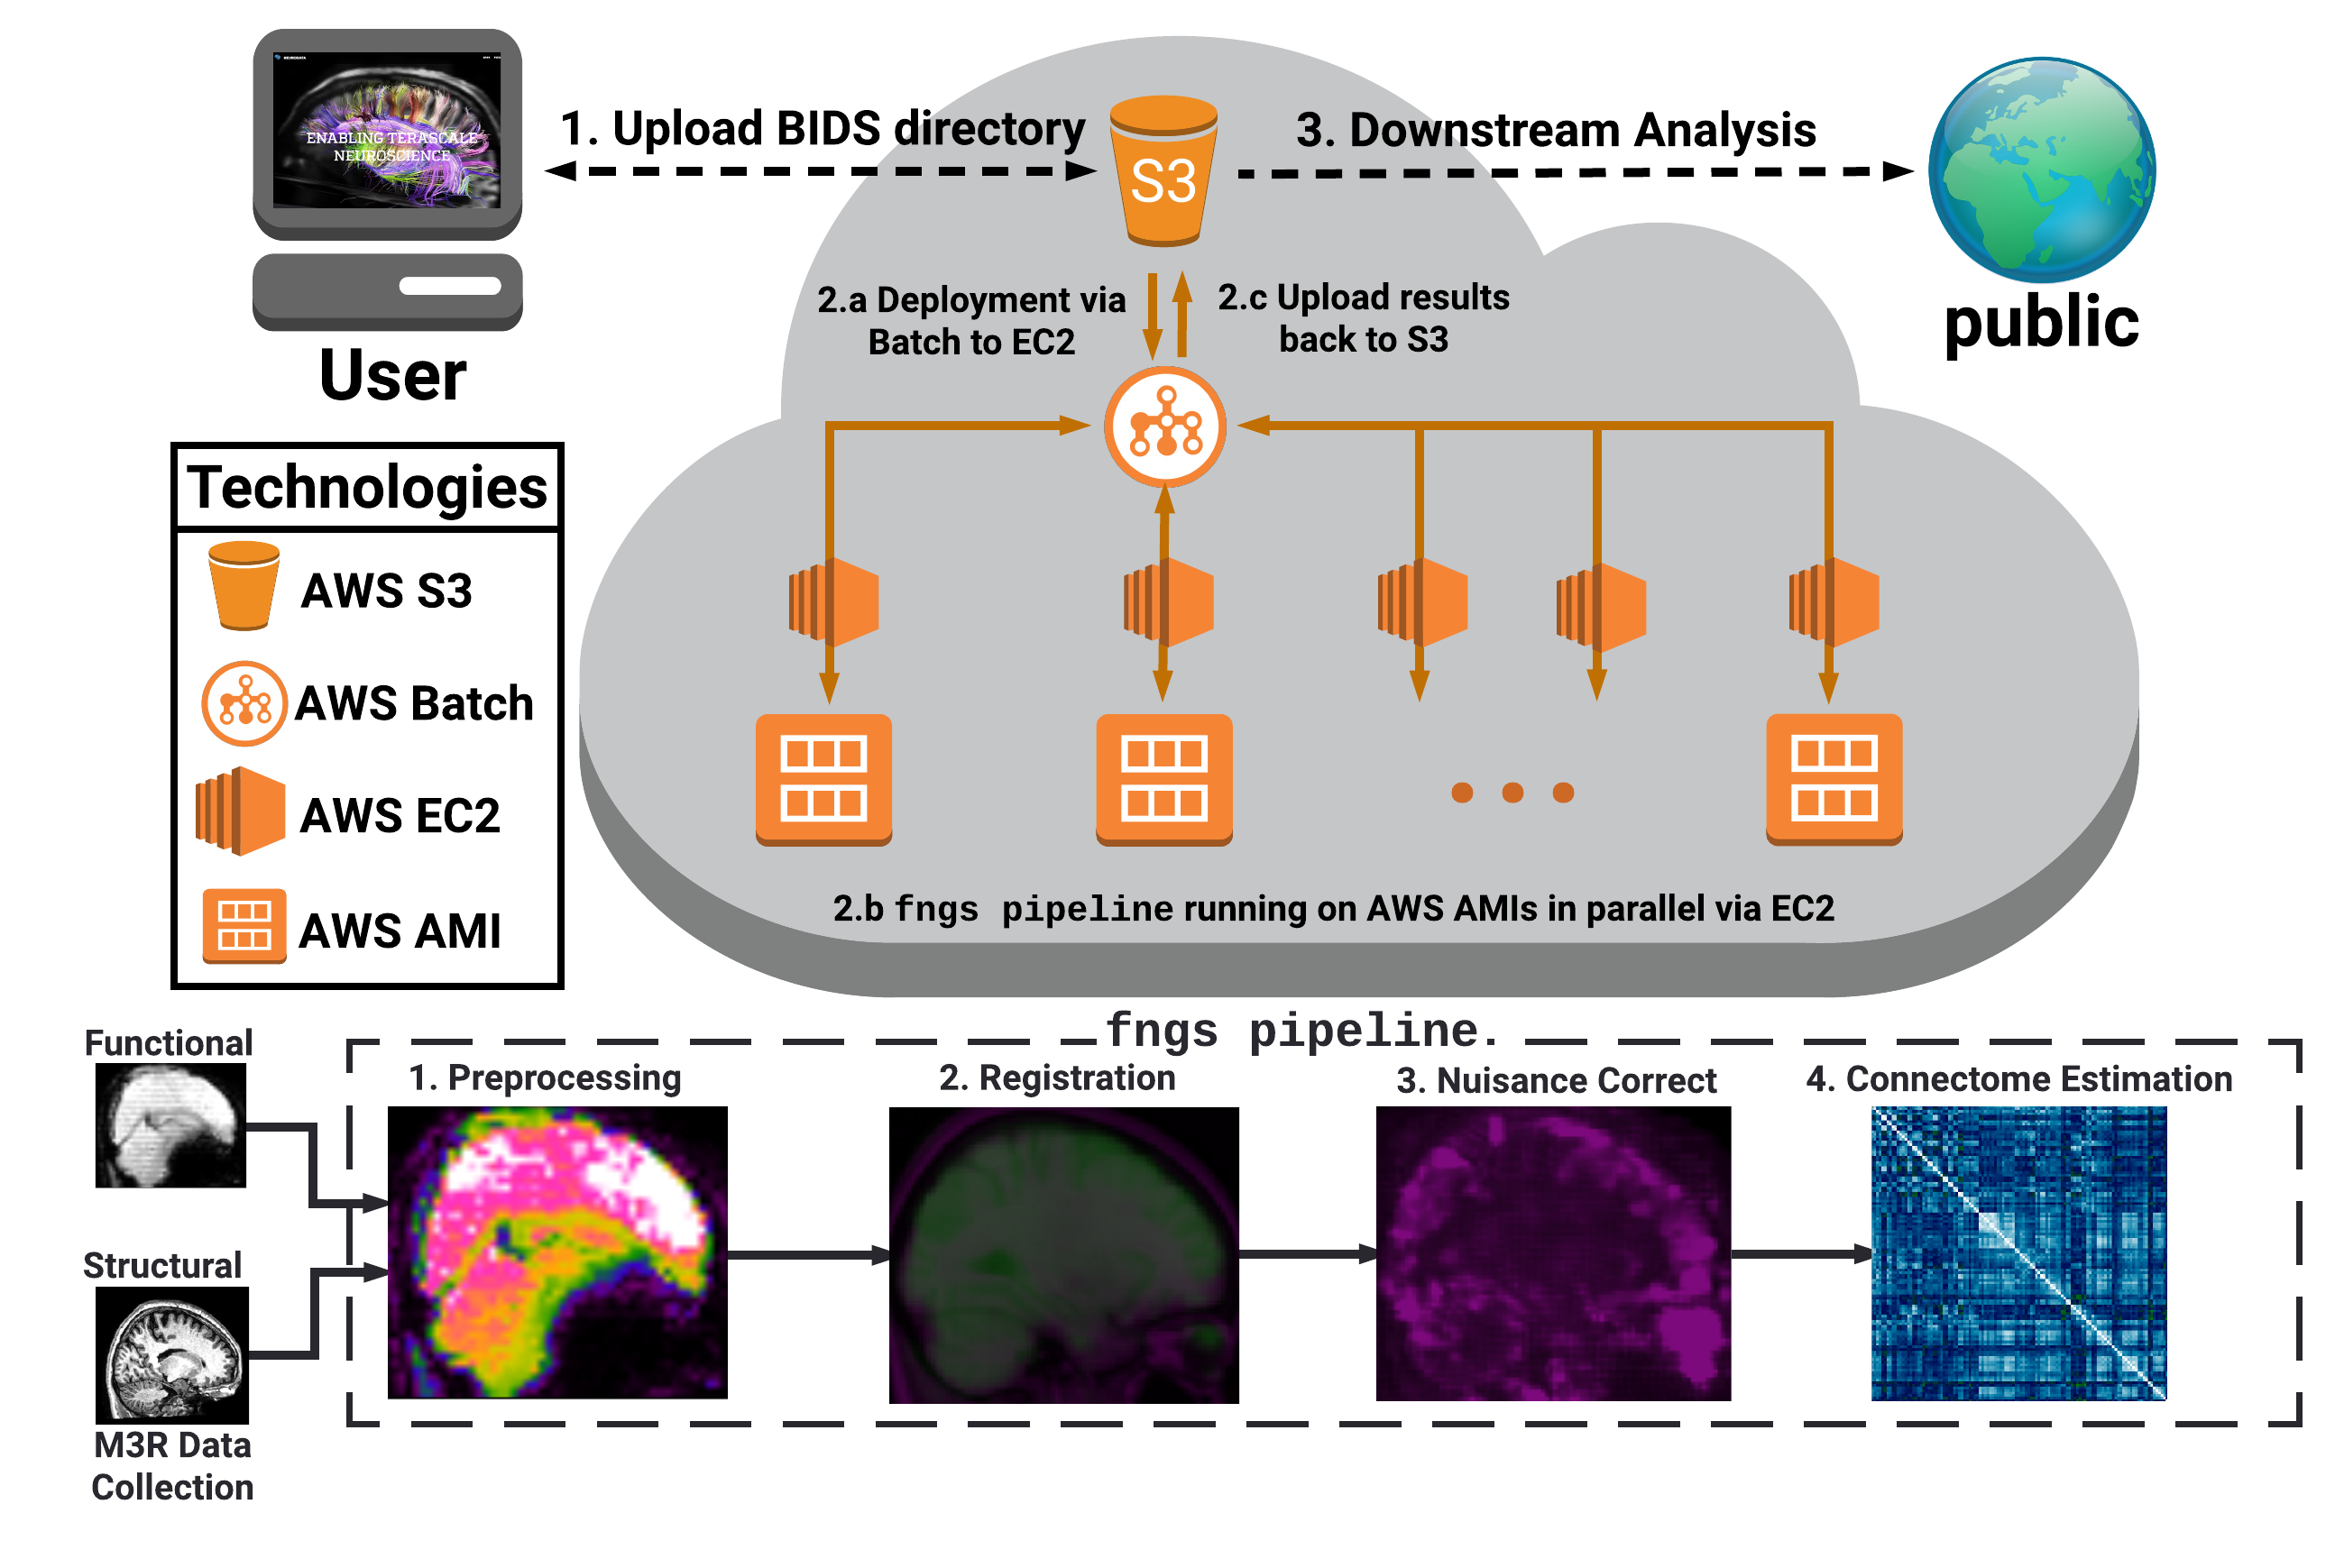
\includegraphics[width=\textwidth]{../../figs/fngs-workflow.png}
\end{subfigure}
\caption{\textbf{FNGS workflow}. The deployment workflow for the FNGS pipeline. Users provide a directory according to the BIDs spec to the FNGS cloud controller locally via the docker container at (1). The data is uploaded directly to AWS S3 cloud drives. The controller then initiates the Batch deployment procedure at (2.a), which interfaces between S3 and EC2 cloud computers to provide the MRI scans to EC2 instances pre-loaded with the FNGS pipeline for analysis. After the scans are finished being analyzed on the EC2 instances at (2.b), the results are then re-uploaded back to the S3 cloud drive at (2.c). The user can then navigate to the S3 cloud drive for downstream analyses.}
\label{fig:fngs-workflow}
\end{cframed}
\end{figure}

\end{document}
